\section{Applikationslaget}
Applikationslaget er det højeste lag i strukturen, og kan betragtes som brugerens interface til resten af programmet. Her adskiller applikationslaget sig fra de andre lag. De andre lag yder services til højere lag, med henblik på at skabe den ønskede forbindelse. Applikationslaget yder imidlertid ikke services til brugeren, og kan således nemt udskiftes med en alternativ applikation. Det kræver blot, at brugerens indtastede information kan konverteres til et format, der kan transporteres af de lavere lag.
	Derfor kommer applikationslaget hovedsageligt til at beskæftige sig med konvertering mellem formater, som hhv. brugeren og transportlaget skal benytte. Som primært fokus skal der udvikles en chat-klient, og af denne årsag kommer dataen på applikationslagsniveau til at være strenge af tekst.
	
	
\begin{figure}[h]
\centering
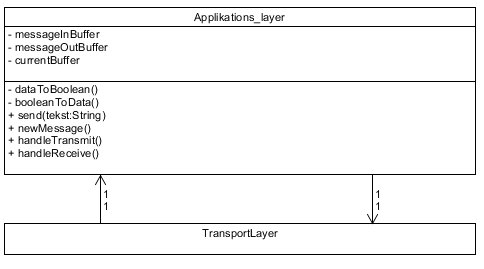
\includegraphics[scale=0.6]{Billeder/ApplicationLayerDesignClass.PNG}
\caption{Uddrag af designklassediagram med applikationslagets essentielle metoder og attributter}
\label{fig:AppLayerDesign}
\end{figure}
	
\subsection{Afsender}
Afsenderens applikationslag har fået tildelt ansvaret for at kunne acceptere et tekst-input fra en chat-bruger. Dette tekst-input skal placeres i en buffer som transport-laget kan tilgå, i et format som transportlaget kan arbejde med. 

\subsubsection{Opløsning i bits}
Der er tidligere er foretaget valg om, at de nedre protokoller arbejder bit-orienteret. Transportlaget opererer under en antagelse om, at al data som kommer fra applikationslaget, skal være en strøm af binære værdier. Hver karakter i strengen skal opløses på 8 bit, da dette muliggør benyttelse af extended ASCII.

\subsubsection{Buffere}



\subsection{Modtager}

\subsubsection{•}
\subsubsection{•}